\documentclass[12pt,a4paper]{article}

\usepackage[utf8]{inputenc}
\usepackage{ctex}
\usepackage{amsmath,amsfonts,amssymb}
\usepackage{abstract,appendix}
\usepackage{makeidx,hyperref}
\usepackage{graphicx,epsfig,subfig}
\usepackage{geometry}
\usepackage{xcolor}

\geometry{scale=0.8}

%\setlength{\lineskip}{\baselineskip}
\setlength{\parskip}{0.5\baselineskip}

\title{Anderson局部化实验报告6}
\author{sis-flag}
\date{\today}

\begin{document}

\section{聚集到边界的概率}

研究特征值问题,定义在$[0,1]^d$上。
\begin{align*}
-\Delta u + K V u = \lambda u \qquad \mathbf{x} \in \Omega \\
\frac{\partial u}{\partial n} + h u = 0 \qquad \mathbf{x} \in \partial \Omega
\end{align*}

研究$V(x)$为Bernoulli分布的情况。\textbf{它以概率$p$取值为0,概率$1-p$取值为1。}

一维情况下,对于某个特征函数$u(x)$,定义它聚集到边界的“程度”
为$$ Pb = \frac{\max\{|u(0)|, |u(1)|\}}{\max_{x \in \Omega} |u(x)|} $$

二维情况下,定义它localize到边界的“程度”为
$$ Pe = \frac{\max_{x \in \partial\Omega} |u(x)|}{\max_{x \in \Omega} |u(x)|} $$
同样可以定义localize到角落的“程度”为
$$ Pc = \frac{\max\{|u(0,0)|, |u(0,1)|, |u(1,1)|, |u(1,0)|\}}{\max_{x \in \Omega} |u(x)|} $$

在Dirichlet边界下,这些都是0。在导数边界条件下,随着$V(x)$随机生成,这些量就是一些和$K,p,h$有关的随机变量。取值在0到1之间。下面研究这个随机变量的分布随参数的变化。

这里\textbf{只画出了最小特征值对应的特征函数},其它较小特征值的规律和它是一样的。

一维情况下,区间分为$20$段。二维情况下,区域被分成$10 \times 10$的方格。

之前的样本点只有100个,结果不是很精确。这里在每种情况下求解了1000个特征值问题。

\newpage
\subsection{关于h的变化}

\paragraph{模拟结果}

集中在边界的程度随$h$的变化如图\ref{fh}。图中参数为$p=0.5, K=10^3$。
\begin{figure}[h]
\centering
\subfloat[一维]{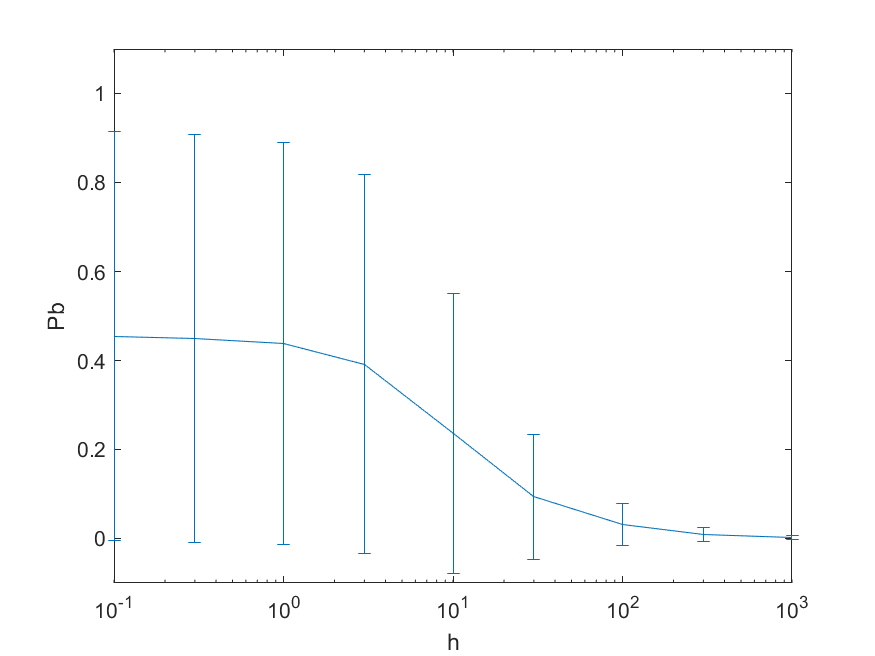
\includegraphics[width=0.3\linewidth]{hb}}
\subfloat[二维(边)]{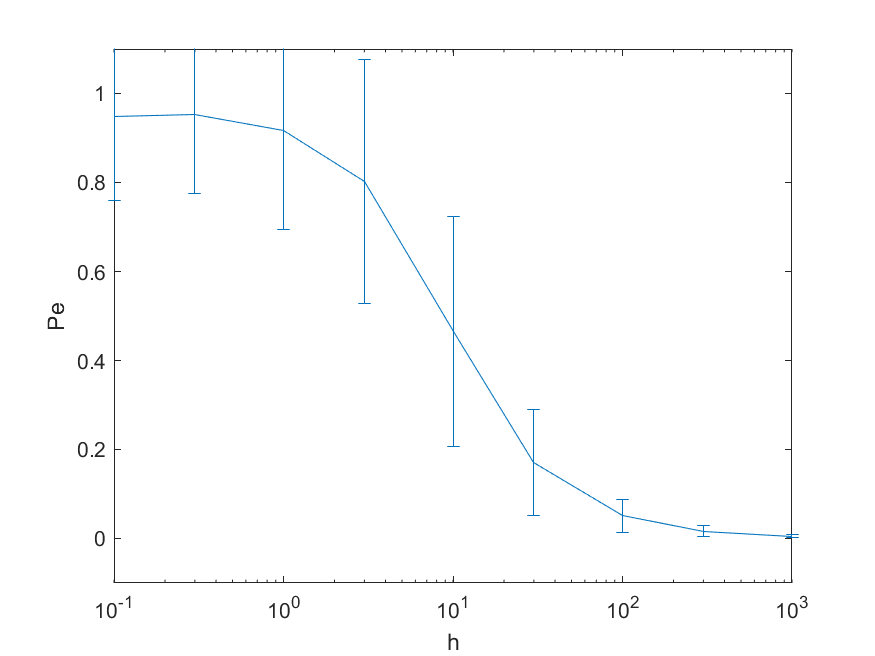
\includegraphics[width=0.3\linewidth]{he}}
\subfloat[二维(角)]{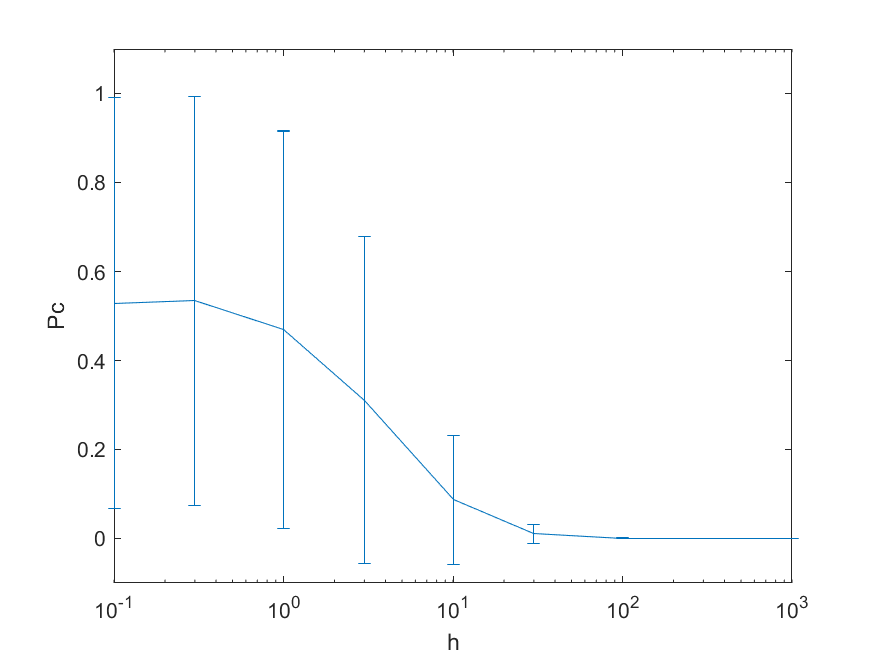
\includegraphics[width=0.3\linewidth]{hc}}
\caption{实验结果}
\label{fh}
\end{figure}

从图中可以看出,集中到边界的程度随$h$都是下降的。而且一维情况下没有二维情况下的剧烈。这和我们的理论相符。因为h越小越接近Neumann边界条件,而h越大越接近于Dirichlet边界条件。一维情况下不剧烈是因为一维情况下,边界附近$V(x)$为0的概率较小,而二维情况下这个概率就大大增加了。

\paragraph{理论分析}

无论其它参数如何变化,在$h$趋于无穷时,方程趋于Dirichlet边界条件,此时聚集到边界的程度趋于0,这一点在所有的模拟结果中都很明显。

在$h$趋于0时,方程趋于Neumann边界条件,情况比较复杂,我们只能分析$K$足够大时候的情况。
根据前面的结果,$K$很大时,Neumann边界条件下,特征函数会聚集到子区域特征值最大的地方。二维情况下的子区域特征值难以分析,一维情况下子区域特征值就是边界对称之后最长的一段。

\textbf{\color{blue} 目前还算不出“最长的一段位于边界”这个概率的表达式。}

\subsection{关于p的变化}

\paragraph{模拟结果}

集中在边界的程度随$p$的变化如图\ref{fp1}。图中参数为$h=1$,一维情况下$K=10^3$,二维情况下$K=10^4$。
\begin{figure}[h]
\centering
\subfloat[一维]{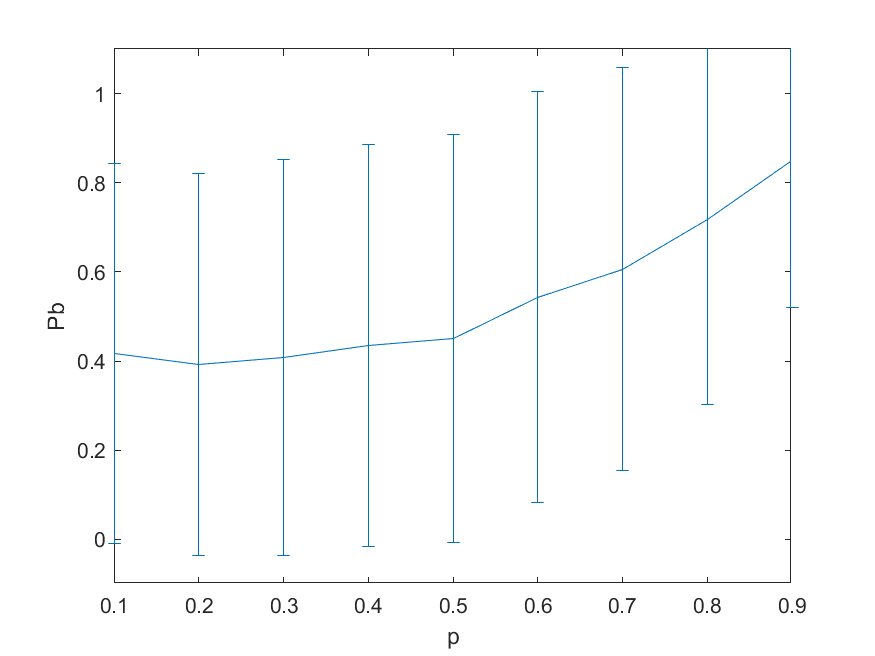
\includegraphics[width=0.3\linewidth]{pb1}}
\subfloat[二维(边)]{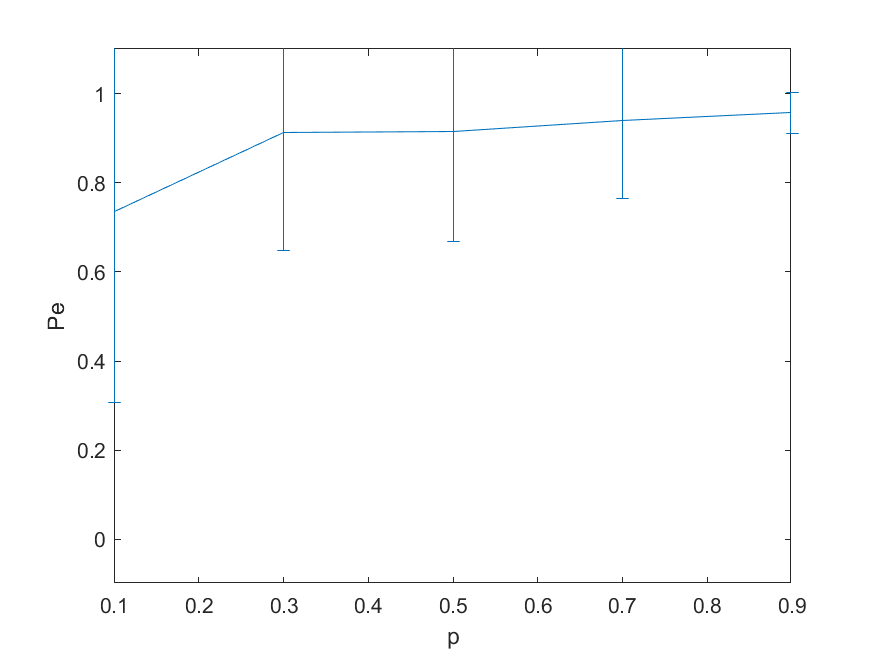
\includegraphics[width=0.3\linewidth]{pe2}}
\subfloat[二维(角)]{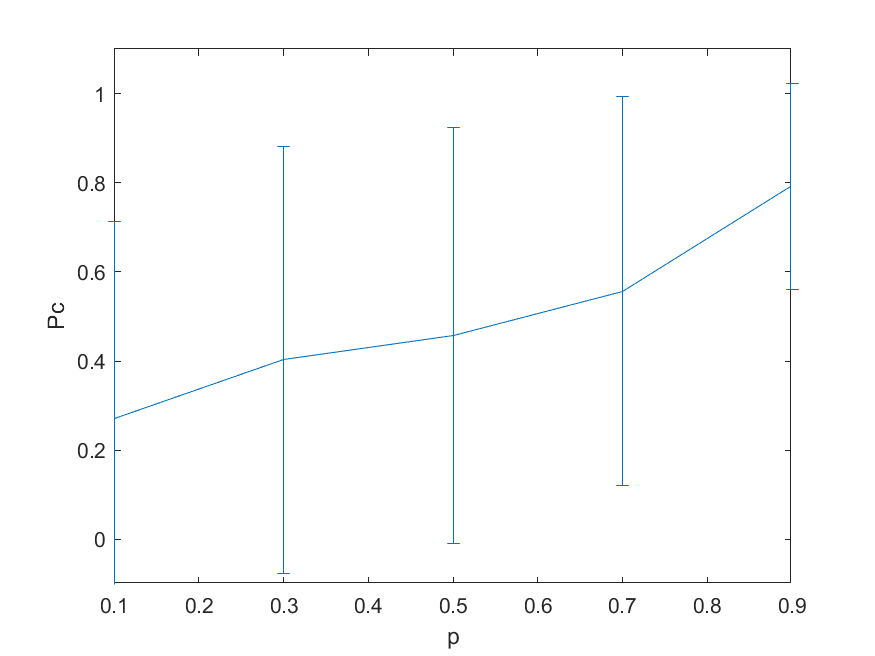
\includegraphics[width=0.3\linewidth]{pc2}}
\caption{实验结果}
\label{fp1}
\end{figure}

从图中可以看出,此时集中到边界的程度随$p$是上升的。

我们换一组参数,得到图\ref{fp2}。图中参数为$h=100$,一维情况下$K=10^3$,二维情况下$K=10^4$。
\begin{figure}[h]
\centering
\subfloat[一维]{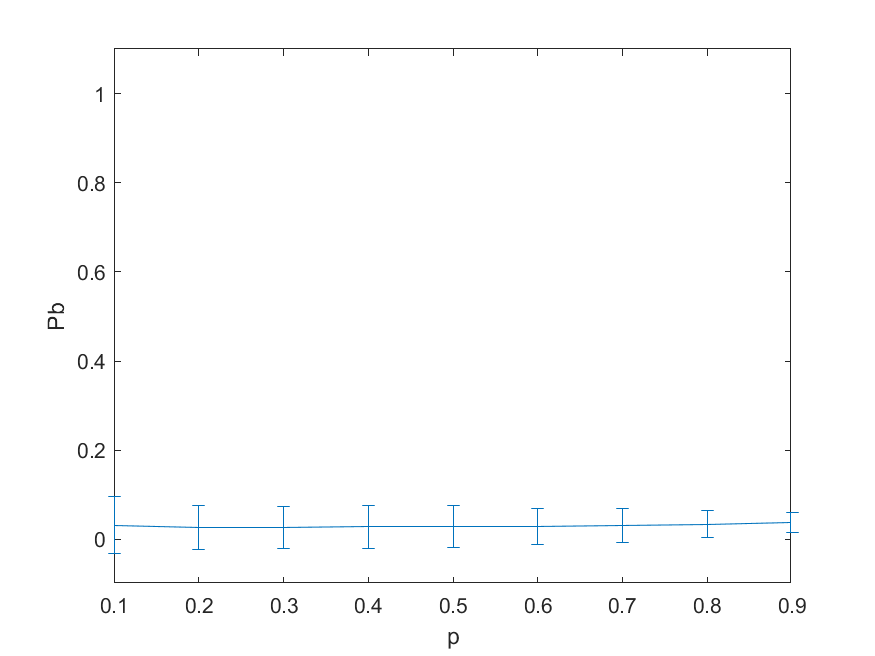
\includegraphics[width=0.3\linewidth]{pb2}}
\subfloat[二维(边)]{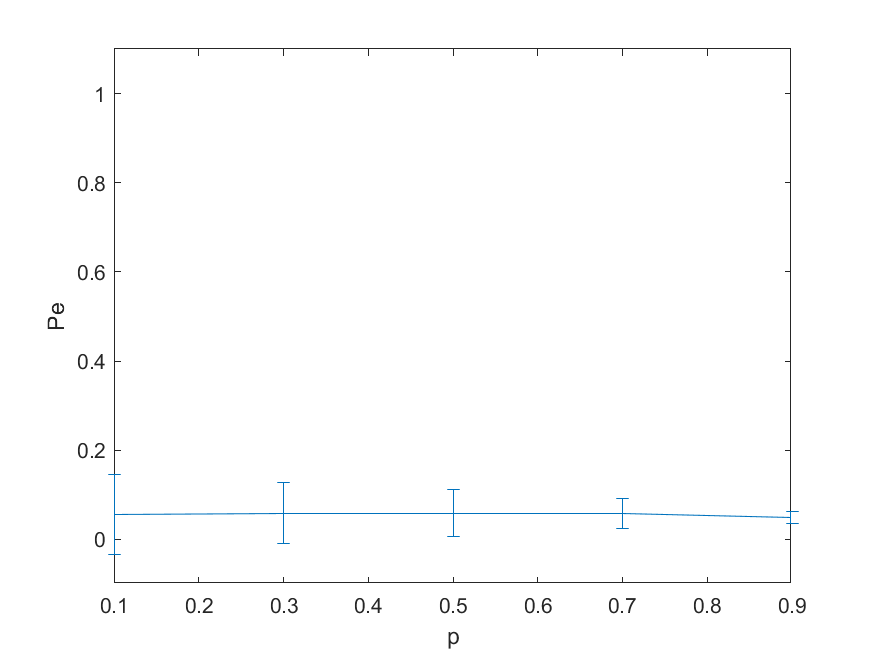
\includegraphics[width=0.3\linewidth]{pe1}}
\subfloat[二维(角)]{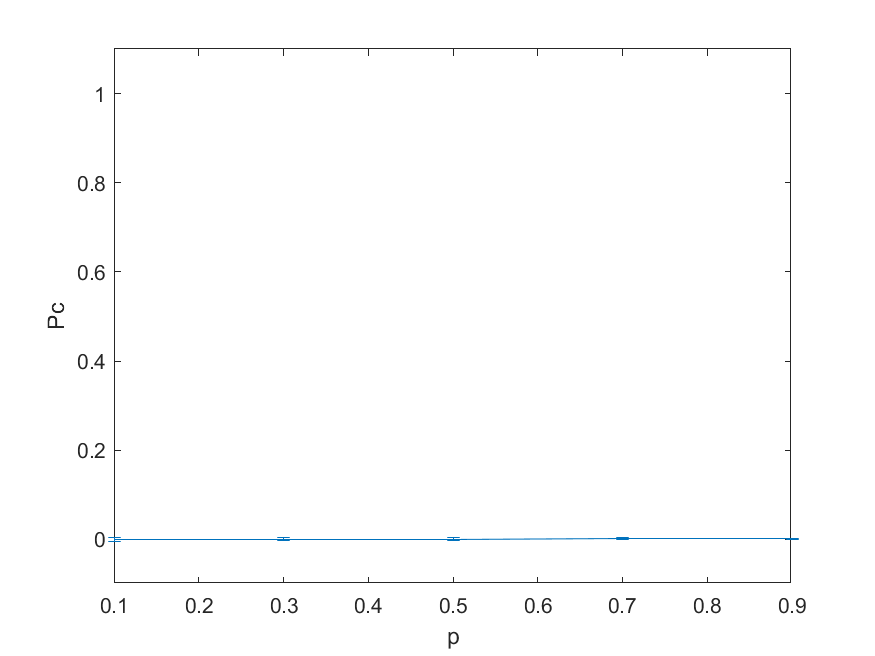
\includegraphics[width=0.3\linewidth]{pc1}}
\caption{实验结果}
\label{fp2}
\end{figure}

从图中可以看出,当$h$很大的时候,方程接近于Dirichlet边界条件,集中到边界的程度接近于0,此时和参数$p$就没什么关系了。

\paragraph{理论分析}

在$p$等于1的时候,$V(x)$恒为0,特征函数就是于常数。此时按照上面的指标,集中到边界的程度为1。在$p$等于0的时候,$V(x)$恒为$K$,特征函数集中到边界的程度由$h$决定。

%分析特征值问题
%\begin{align}
%-\triangle u + K u = \lambda u \qquad x \in \Omega \\
%\frac{\partial u}{\partial n} + h u = 0 \qquad x \in \partial \Omega
%\end{align}
%这个东西看起来挺简单的,但是我不知道它的解析解。数值结果是表明,$h=1$的时候,一维情况下聚集到边界的程度为$0.7941$,根据对称性,二维的函数可以表示为一维的相乘,聚集到边界的程度为$0.7941$,聚集到角上的程度为$0.6306$。这个数字和模拟结果对不上,不知道为什么。。。

图\ref{fpf}中展示了不同$K$下,程度随$p$变化的情况,取的点比较少。\textbf{\color{blue} 看起来这个问题可能比我们想的要复杂。}
\begin{figure}[h]
\centering
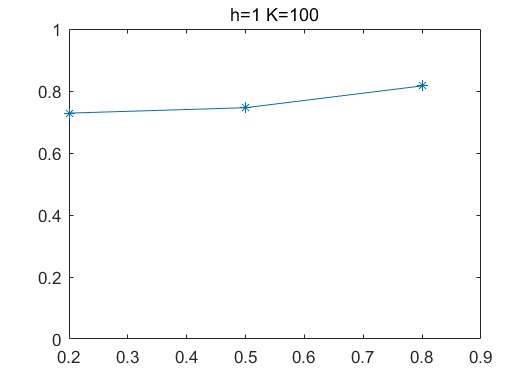
\includegraphics[width=0.24\linewidth]{pbf1}
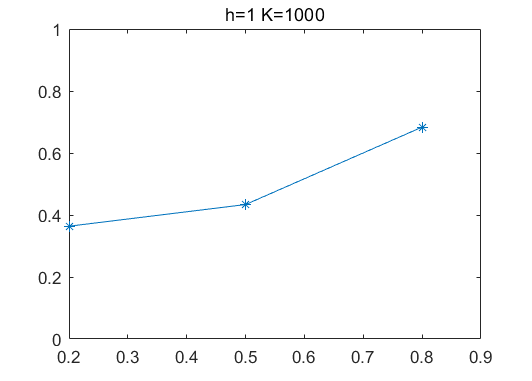
\includegraphics[width=0.24\linewidth]{pbf2}
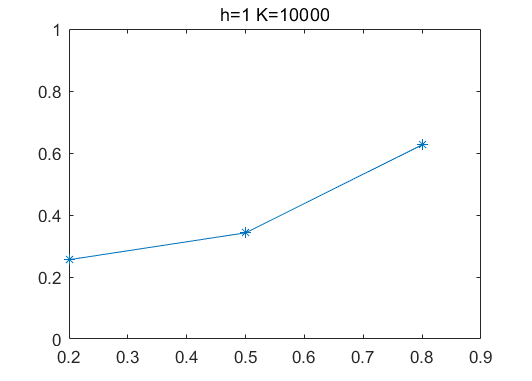
\includegraphics[width=0.24\linewidth]{pbf3}
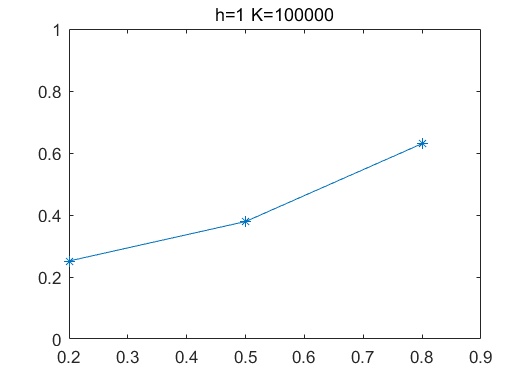
\includegraphics[width=0.24\linewidth]{pbf4}
\caption{实验结果}
\label{fpf}
\end{figure}

%在$p$很小的时候,我们可以近似地认为区间内没有两段连在一起取值为0的小段。在$K$很大的时候,我们可以近似认为特征函数在$V(x)$取值为1的时候为0。在边界的两段取值为1的时候,可以近似认为集中到边界的程度是0。取值为0的时候,可以近似认为一定会集中到边界。

\subsection{关于K的变化}

集中在边界的程度随$K$的变化如图\ref{fk1}。图中参数为$h=1, p=0.5$。
\begin{figure}[h]
\centering
\subfloat[一维]{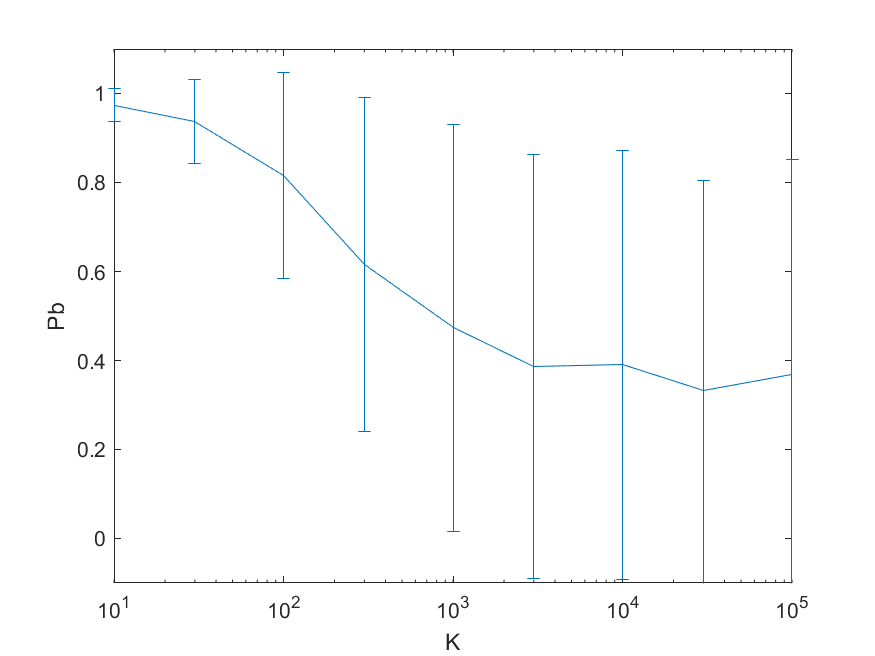
\includegraphics[width=0.3\linewidth]{kb1}}
\subfloat[二维(边)]{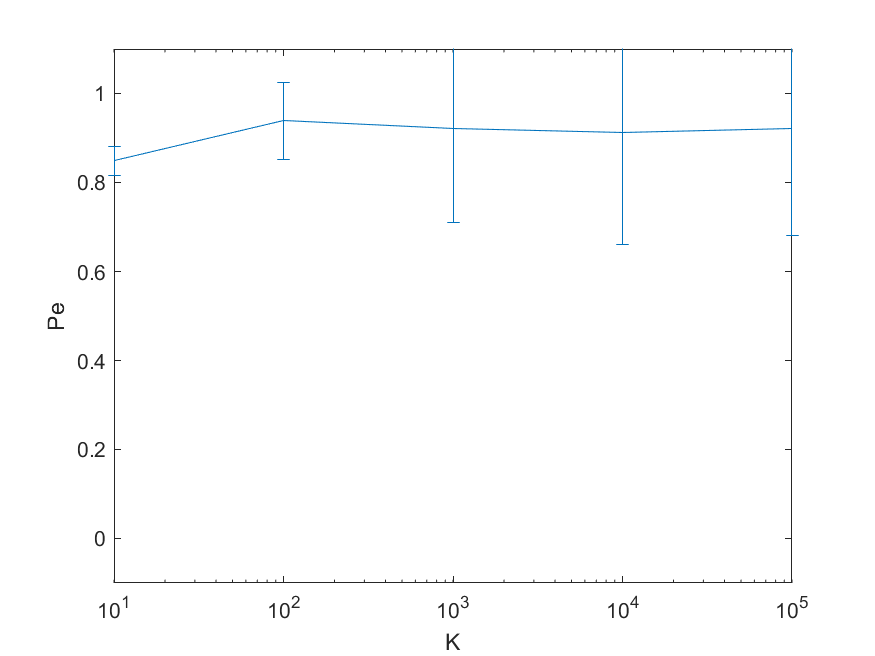
\includegraphics[width=0.3\linewidth]{ke1}}
\subfloat[二维(角)]{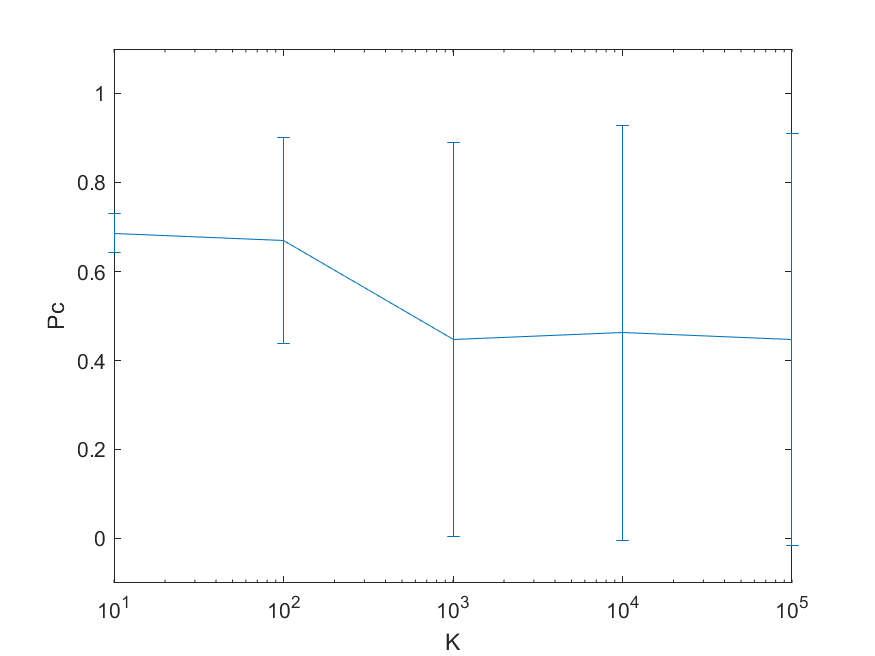
\includegraphics[width=0.3\linewidth]{kc1}}
\caption{实验结果}
\label{fk1}
\end{figure}

从图中可以看出,当$K$接近0的时候,特征函数接近常数,一定会聚集到边界。随着$K$逐渐增大,特征函数会逐渐产生聚集在某处的峰,此时可能不会聚集到边界。

\textbf{\color{blue} 对于二维情况,我们实在不知道该怎么解释。}在$K$较大,已经产生localize现象的时候,我们可以看出,$K$对结果影响不大。在$K$较小的时候,localize现象还没有产生,分析起来比较困难。

图\ref{bk}中画出了某一个势函数下,不同的$K$对应的最小特征函数。可以看出,在一维的时候,localization现象比较明显,而二维的时候,只有$K$很大的时候才有这种现象。在二维$K$不大不小的时候,什么都可能发生,很难分析。
\begin{figure}[h]
\centering
\subfloat[]{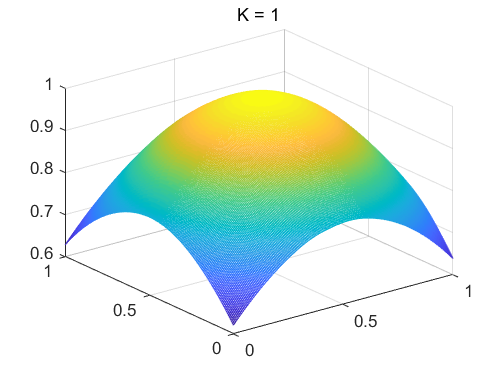
\includegraphics[width=0.24\linewidth]{bk1}}
\subfloat[]{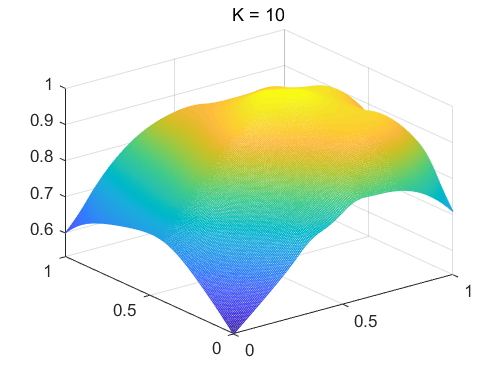
\includegraphics[width=0.24\linewidth]{bk2}}
\subfloat[]{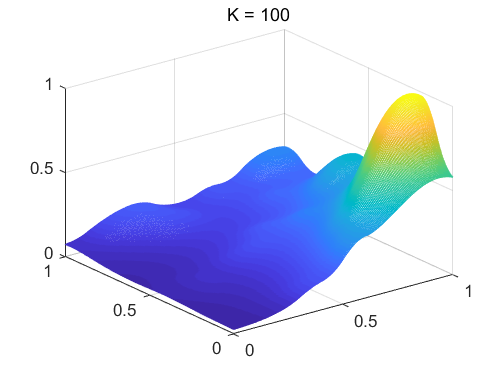
\includegraphics[width=0.24\linewidth]{bk3}}
\subfloat[]{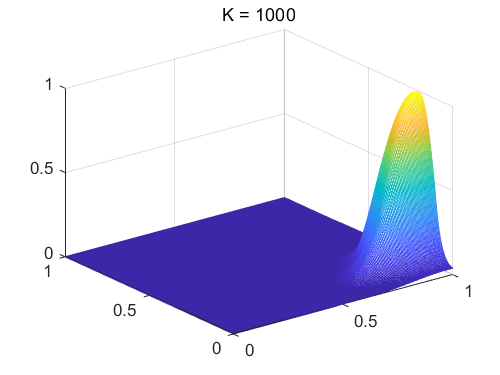
\includegraphics[width=0.24\linewidth]{bk4}}
\caption{不同的K}
\label{bk}
\end{figure}

我们换一组参数,得到图\ref{fk2}。图中参数为$h=100, p=0.5$。
\begin{figure}[h]
\centering
\subfloat[一维]{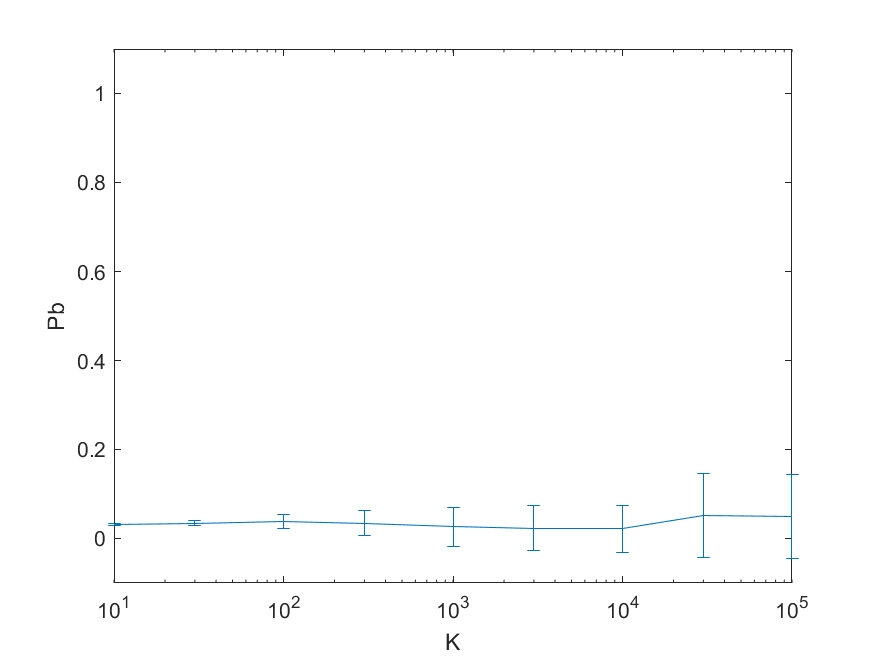
\includegraphics[width=0.3\linewidth]{kb2}}
\subfloat[二维(边)]{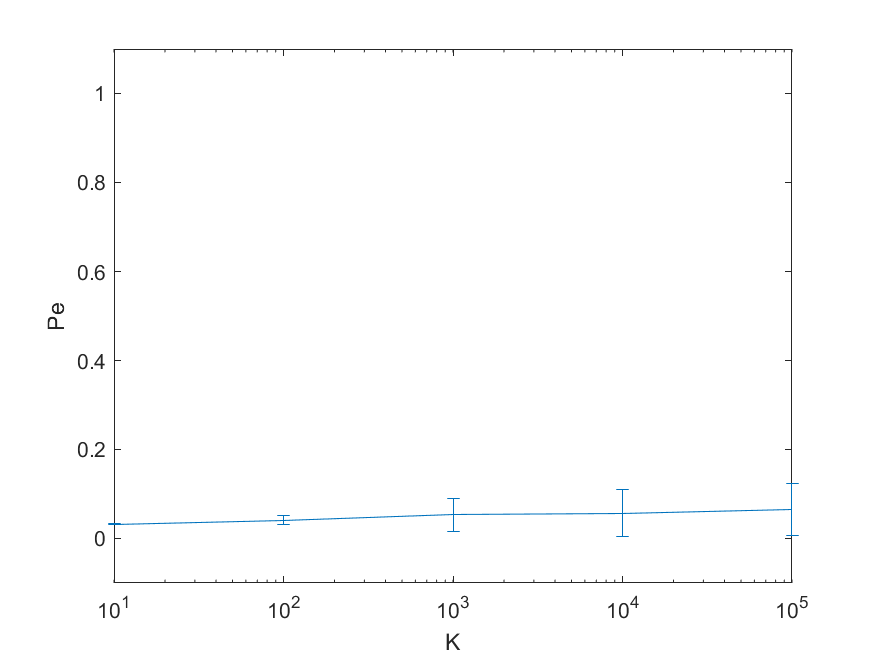
\includegraphics[width=0.3\linewidth]{ke2}}
\subfloat[二维(角)]{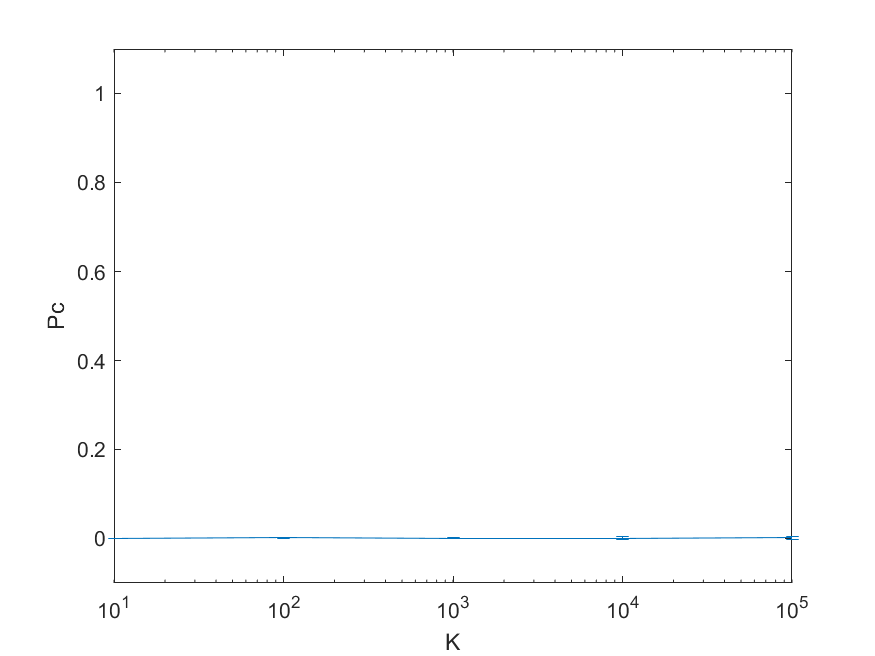
\includegraphics[width=0.3\linewidth]{kc2}}
\caption{实验结果}
\label{fk2}
\end{figure}

从图中可以看出,当$h$很大的时候,它和参数$K$也没什么关系。

\newpage
\section{相变}

这里我们考虑一维的情况。势函数取成:$N_2/2$个1 + $N_1$个0 + $N_2$个1 +  $N_3$个0 +  $N_4$个1 +  $N_5$个0 + :$N_2/2$个1。其中$\max\{N_3, N_5\} < N_1 < N_3 + N_5$(两边差不多长),$N_4 < \min\{N_3, N_5\} / 2$(被吃掉的部分要足够短),$N_2 > N_1+ N_3 + N_4 + N_5$(中间的分隔要足够长)。边界为周期边界。总长度$N = N_2 + N_1 + N_2 + N_3 + N_4 + N_5$。
\begin{figure}[h]
\centering
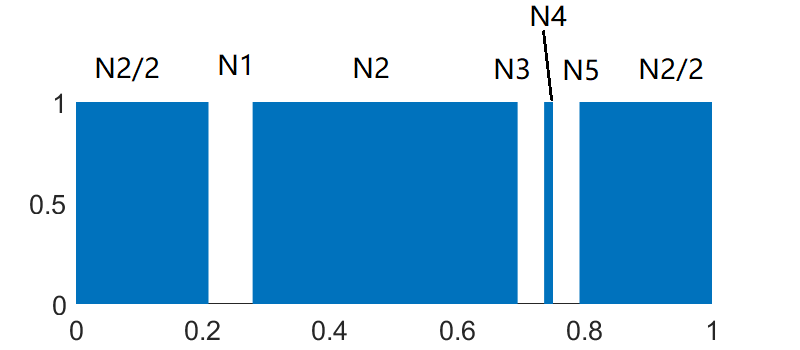
\includegraphics[width=0.7\linewidth]{N}
\caption{示意图}
\end{figure}


取$N=(5,24,3,1,3)$,
画出不同$K$值下的第一个,第二个特征函数,和landscape如图\ref{f3}。可以看出,landscape变化不大,但是特征函数localize的位置发生很大变化。
\begin{figure}[h]
\centering
\subfloat[u1]{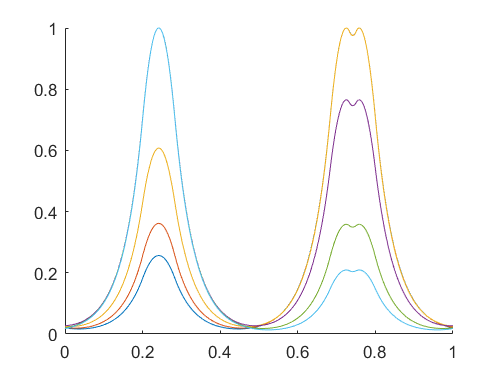
\includegraphics[width=0.3\linewidth]{U1}}
\subfloat[u2]{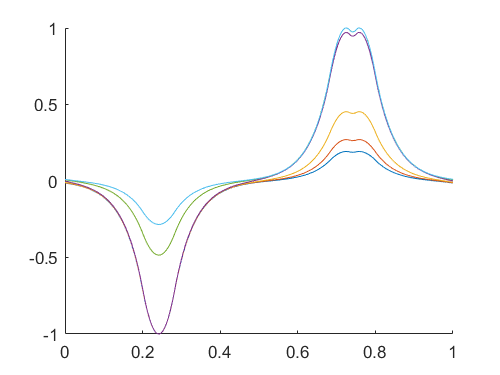
\includegraphics[width=0.3\linewidth]{U2}}
\subfloat[w]{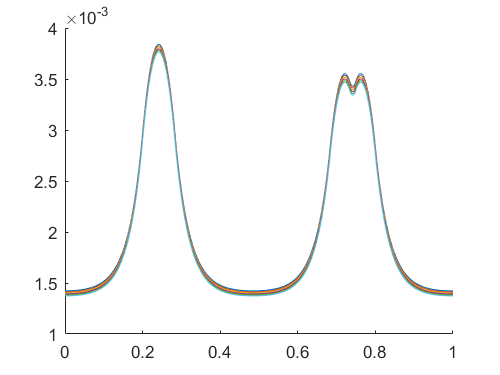
\includegraphics[width=0.3\linewidth]{W}}
\caption{模拟结果}
\label{f3}
\end{figure}

这里最小的特征函数可能出现两个峰,定义$F$为左峰高度除以左右两个峰高度之和。下面的图\ref{f4}里画出了第一个,第二个特征函数,和landscape的$F$随$K$的变化。横轴是K,纵轴是F。
\begin{figure}[h]
\centering
\subfloat[u1]{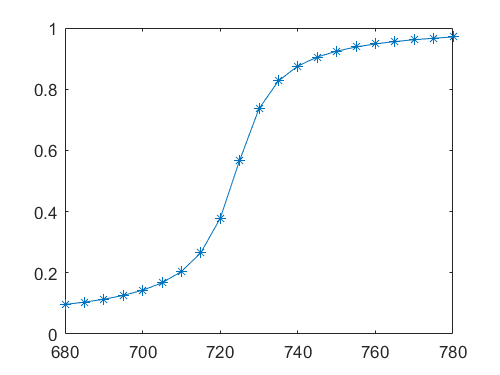
\includegraphics[width=0.3\linewidth]{FU1}}
\subfloat[u2]{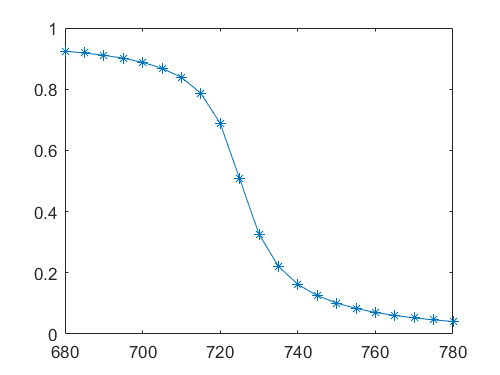
\includegraphics[width=0.3\linewidth]{FU2}}
\subfloat[w]{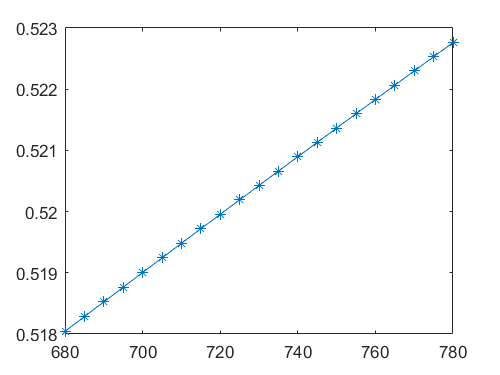
\includegraphics[width=0.3\linewidth]{FW}}
\caption{模拟结果}
\label{f4}
\end{figure}

可以看出,landscape的峰高度比随K大致是线性的,变化范围很小。u1和u2会有“相变”的现象。而且u1和u2呈现明显的负相关,相变的位置几乎相同。它们的F加起来近似等于1。这一点可以通过正交性解释。前两个特征函数一定是正交的,也就是说相乘之后积分为0。因此第一个特征函数有两个峰,而且峰值全是大于0的时候,第二个特征函数的两个峰必定一正一负,而且高度的大小和第一个相反。这里的解释只是一个定量的解释,在模拟中,$F1$和$F2$相加并不是精确等于1的。

对于特征值,图\ref{f5}中画出了前几个特征值随K变化的图像。横轴是K,纵轴是特征值。
localize到左边的特征函数对应一个特征值,localize到右边的对应一个特征值。它们随K增加而增长的变化速率不一样。
由于我们关心“最小”特征值对应的特征函数,当一个特征值和另一个相等的时候,“最小”的特征值就从一个变成了另一个,从而发生了相变。
后面的特征值和两个最小的特征值之间有很大的一段间隔,它们对相变几乎没什么影响。
\begin{figure}[h]
\centering
\subfloat[特征值]{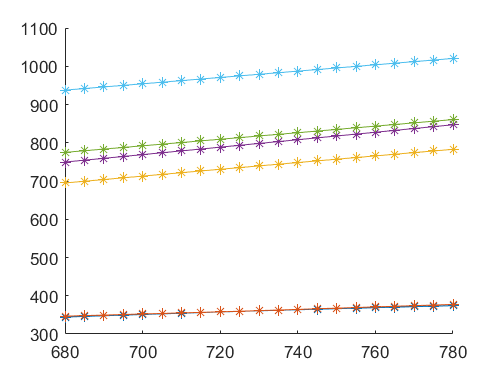
\includegraphics[width=0.3\linewidth]{Flam}}
\subfloat[特征值放大图]{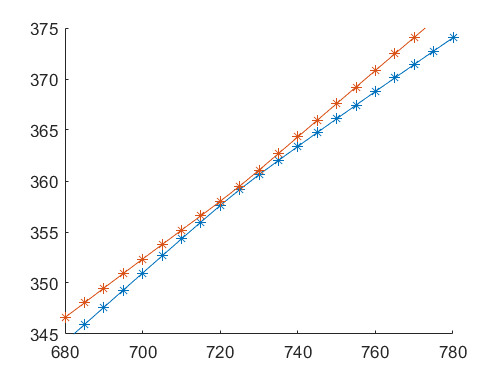
\includegraphics[width=0.3\linewidth]{Flam2}}
\caption{模拟结果}
\label{f5}
\end{figure}

下面我们只研究最小特征值对应特征函数的相变现象。

这里对变量进行归一化,定义
$$ L_1 = \frac{N_1}{N}, \quad L_2 = \frac{2 N_2}{N}, \quad L_3 = \frac{N_3}{N}, \quad L_4 = \frac{N_4}{N}, \quad L_5 = \frac{N_5}{N} $$
这里满足$L_1+L_2+L_3+L_4+L_5 = 1$,它们分别对应问题中对应某一段的区间长度。

这五个变量中共有4个自由度。后面我们分别拟合这4个变量和相变点之间的关系。

\subsection{模拟结果}

下面我们做了更多的模拟,得到了不同$N$下的相变阈值,以及阈值附近相变的剧烈程度。表\ref{t1}中是用二分法求的。
后面的a和b是用公式
$$ F - 0.5 = b(K - K_c)^a $$
拟合得到的相变临界指数。这里的临界指数都是1,说明这里的相变比较平缓,不是那种剧烈的相变。

表中展示了更多结果。结果数量很多,表里只有一部分。从这里可以看出,\textbf{换成周期边界条件之后,$N_3$和$N_5$的地位完全等同了!}
\begin{table}[h]
\centering
\begin{tabular}{ccccccccccc}
\hline
$N_1$ & $N_2$ & $N_3$ & $N_4$ & $N_5$ & K(F=0.2) & K(F=0.5) & K(F=0.8) & a & b & $F'(K)$ \\
\hline
3 & 10 & 2 & 1 & 2 & 413.648 & 448.785 & 467.804 & 0.990349 & 0.00977886 & 0.0096554 \\
3 & 14 & 2 & 1 & 2 & 744.921 & 749.735 & 753.546 & 1.0029 & 0.0553361 & 0.0551021 \\
3 & 18 & 2 & 1 & 2 & 1120.48 & 1121.27 & 1121.92 & 1.00228 & 0.331664 & 0.329056 \\
4 & 14 & 2 & 1 & 3 & 485.277 & 506.996 & 521.789 & 0.994986 & 0.0135875 & 0.0135081 \\
4 & 16 & 2 & 1 & 3 & 610.77 & 620.751 & 628.73 & 1.0015 & 0.0266872 & 0.0266278 \\
4 & 20 & 2 & 1 & 3 & 878.578 & 880.924 & 883.011 & 1.00163 & 0.10729 & 0.106806 \\
4 & 14 & 3 & 1 & 2 & 485.277 & 506.996 & 521.789 & 0.994986 & 0.0135875 & 0.0135081 \\
4 & 16 & 3 & 1 & 2 & 610.77 & 620.751 & 628.73 & 1.0015 & 0.0266872 & 0.0266278 \\
4 & 20 & 3 & 1 & 2 & 878.578 & 880.924 & 883.011 & 1.00163 & 0.10729 & 0.106806 \\
4 & 13 & 3 & 1 & 3 & 1089.76 & 1090.34 & 1090.8 & 1.00172 & 0.457853 & 0.454671 \\
4 & 19 & 3 & 1 & 3 & 1912.53 & 1912.54 & 1912.55 & 0.989933 & 21.1165 & 22.5528 \\
\hline
\end{tabular}
\caption{模拟结果}
\label{t1}
\end{table}

定义左右两个峰一样高$F=0.5$时为相变点$K_c$。

\subsection{$K_c$和$b$之间的关系}

我们观察到,相变点越大的时候,相变越剧烈。我们首先来验证这个想法,做出临界点$Kc$和临界点导数$b$的散点图,如图\ref{fkb}。可以看出,它们之间有很强的正相关关系。我们尝试用多项式拟合这些散点,得到的关系为
$$ \log(b) = p_2 K_c^2 + p_1 K_c + p_0 \qquad p_2 = -0.49 \times 10^{-6}, p_1 =  0.00612, p_0 = -7.35 $$
虽然这个多项式外推的趋势不太靠谱,但至少在当前范围内精确度比较高。线性模型似乎不能很好的刻画这个趋势。

\textbf{\color{blue} 好像也想不出为什么相变点越大时越剧烈,只是观察到了这样的现象。}

\begin{figure}[h]
\centering
\subfloat[线性拟合]{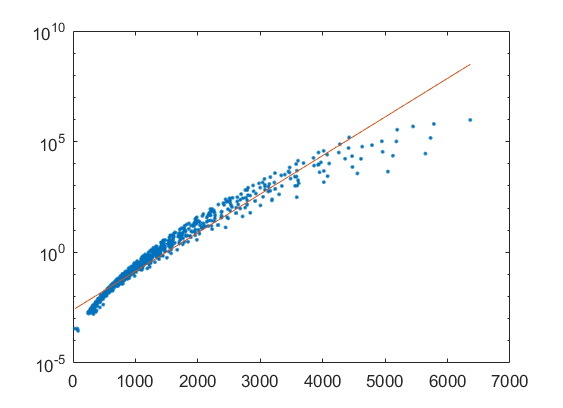
\includegraphics[width=0.4\linewidth]{kcb1}}
\subfloat[二次多项式]{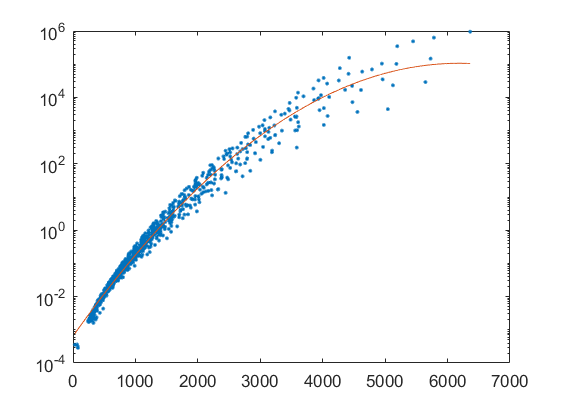
\includegraphics[width=0.4\linewidth]{kcb2}}
\caption{$K_c$-$b$拟合结果}
\label{fkb}
\end{figure}

\subsection{$L_2$和$K_c$之间的关系}

$N_2$对应的区域,作用就是把两段区域分割开。相变的本质是子区域的特征值哪个更大,整个问题是定义在$[0,1]$上的,因此增加$L_2$相当于压缩两个子区域的区间长度,而区间长度的平方是和特征值成反比的。

根据这些分析,我们猜测关系为
$$ \frac{1}{K_c} = A_c (L_1+L_3+L_4+L_5)^2 $$

在以下三组参数对模型进行拟合,得到拟合的参数值和$R^2$如下:
\begin{align*}
N=(5, ?, 3, 1, 3), \quad A_c = 0.0346, \quad R^2 = 1 - 2.6 \times 10^{-6} \quad \text{图中紫色} \\
N=(5, ?, 3, 1, 4), \quad A_c = 0.0112, \quad R^2 = 1 - 1.3 \times 10^{-11} \quad \text{图中红色} \\
N=(7, ?, 5, 1, 5), \quad A_c = 0.0077, \quad R^2 = 1 - 2.6 \times 10^{-15} \quad \text{图中蓝色}
\end{align*}
由于数据是由模拟生成的,而不是从实际测量中获得,所以几乎没有什么误差,$R^2$的值十分接近1也是可以接受的。

图\ref{fn2}中可以看出,拟合结果很好。$A_c$是一个和$N_2$无关的量,它越大代表相变点越小。
\begin{figure}[h]
\centering
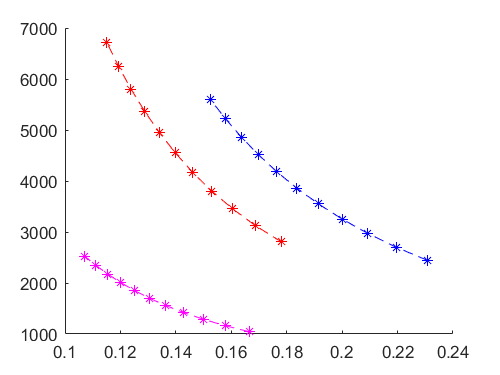
\includegraphics[width=0.4\linewidth]{n2kc}
\caption{拟合结果。横轴:$(L_1+L_3+L_4+L_5)^2$,纵轴:$K_c$}
\label{fn2}
\end{figure}

\subsection{$L_4$和$A_c$之间的关系}

画出$L_4$和$A_c$之间的散点图,我们发现它们近似是线性的关系。

进一步分析发现,如果$N_4$等于0,模型中就不会出现相变。在$N_4$趋近于0的时候,相变点会不断变大,直到无穷,此时$A_c$趋于0,所以线性关系对应的直线一定要过原点。

在$N_4$很大的时候,相变会消失,也就是随着$L_4$的增大,$A_c$会在某个有限的位置趋于无穷。因此这里得到的线性关系只有在$L_4$较小的某个范围内才成立。

我们猜测$N_4$和$A_c$之间的关系为
$$ A_c = B_c L_4 $$

在以下三组参数对模型进行拟合,得到拟合的参数值和$R^2$如下:
\begin{align*}
N=(30, 100, 20, ?, 20), \quad B_c = 0.0.7608, \quad R^2 = 1 - 1.2 \times 10^{-3} \quad \text{图中紫色} \\
N=(20, 80, 15, ?, 15), \quad B_c = 0.4434, \quad R^2 = 1 - 1.6 \times 10^{-3} \quad \text{图中红色} \\
N=(25, 90, 20, ?, 15), \quad B_c = 0.5523, \quad R^2 = 1 - 9.6 \times 10^{-4} \quad \text{图中蓝色}
\end{align*}

图\ref{fn4}中可以看出,拟合结果很好。图中的这些直线都通过原点。
这说明$N_4$越大的时候相变点越小,这和我们的直观相符。
\begin{figure}[h]
\centering
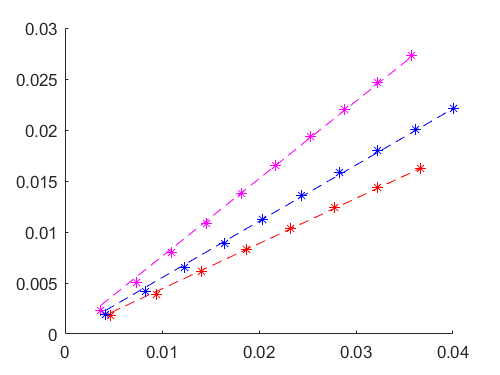
\includegraphics[width=0.4\linewidth]{n4ac}
\caption{拟合结果。横轴:$L_4$,纵轴:$A_c$}
\label{fn4}
\end{figure}

\subsection{$N_4$对应的位置和$B_c$之间的关系}

这里我们保持$N_3+N_4+N_5$整个区间的长度不变,改变$N_4$对应区间在其中的位置。由于$N_3$和$N_5$地位等同,这里的图像有一定的对称性。
下面我们深入分析。在$N_1 > N_3$且$N_1 > N_5$的时候,只要$K$足够大,就一定会发生相变。
而不满足这两个条件的时候,无论如何都不会发生相变。$N_3$或$N_5$靠近$N_1$的时候,相变点就会变大,趋于无穷,此时$A_c$趋于0。

\begin{figure}[h]
\centering
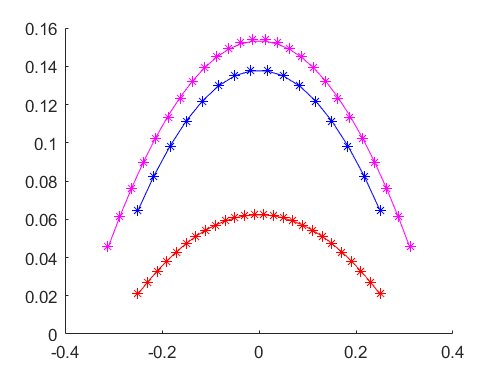
\includegraphics[width=0.4\linewidth]{n3ac}
\caption{对称性示意图。横轴:$L_3-L_5$,纵轴:$B_c$}
\label{fn30}
\end{figure}

根据这些分析,我们猜测关系为
$$ B_c = D_c (L_3 - L_1)(L_5 - L_1) $$

图\ref{fn31}中可以看出问题。图中所展示的关系确实是线性关系,但是常数项不为0,\textbf{\color{blue} 这就和我们的猜测不符,无法进行下去了。}
\begin{figure}[h]
\centering
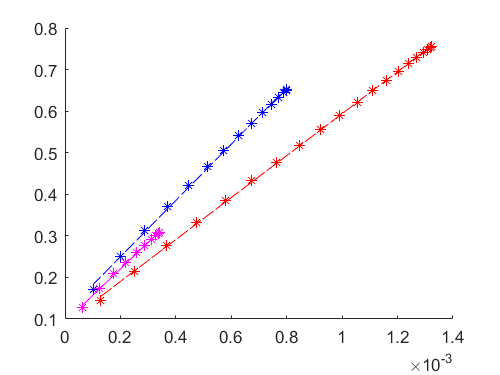
\includegraphics[width=0.4\linewidth]{n3bc}
\caption{拟合结果。横轴:$(L_3 - L_1)(L_5 - L_1)$,纵轴:$B_c$}
\label{fn31}
\end{figure}

%\begin{align*}
%N=(60, 200, ?, 10, 80-?), \quad B_c = 0.0.7608, \quad R^2 = 1 - 1.2 \times 10^{-3} \quad \text{图中紫色} \\
%N=(50, 200, ?, 11, 80-?), \quad B_c = 0.4434, \quad R^2 = 1 - 1.6 \times 10^{-3} \quad \text{图中红色} \\
%N=(50, 200, ?, 10, 70-?), \quad D_c = 0.5523, \quad R^2 = 1 - 9.6 \times 10^{-4} \quad \text{图中蓝色}
%\end{align*}

\subsection{$L_1$和$A_c$之间的关系}

对于$L_1$,同样可以分析出来,如果$L_1$趋近于$\max\{L_3, L_5\}$的时候,模型中就不会出现相变,相变点会不断变大,直到无穷,此时$A_c$趋于0,所以对应的线一定要过原点。
在$L_1$很大的时候,相变会消失,也就是随着$L_1$的增大,$A_c$会在某个有限的位置趋于无穷。

画出$L_1$和$A_c$之间的散点图。如图\ref{fn1}。图中的虚线是假设它们之间具有指数关系得到的。这也是在一定范围内成立的近似。
\begin{figure}[h]
\centering
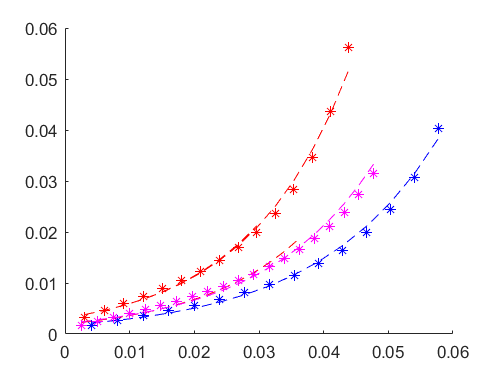
\includegraphics[width=0.4\linewidth]{n1ac}
\caption{拟合结果。横轴:$L_1 - \max\{L_3, L_5\}$,纵轴:$A_c$}
\label{fn1}
\end{figure}

%\begin{align*}
% N=(?, 150, 30, 9, 30), \quad B_c = 0.7608, \quad R^2 = 1 - 1.2 \times 10^{-3} \quad \text{图中紫色} \\
% N=(?, 120, 30, 7, 20), \quad B_c = 0.4434, \quad R^2 = 1 - 1.6 \times 10^{-3} \quad \text{图中红色} \\
% N=(?, 100, 20, 5, 20), \quad D_c = 0.5523, \quad R^2 = 1 - 9.6 \times 10^{-4} \quad \text{图中蓝色}
%\end{align*}

%
%临界点的大小和两个子区域长度的比值之间大概是指数相关的。$N_1$越长相变点越小,这和我们的直观相符。




\end{document}